%%%%%%%%%%%%%%%%%%%%%%%%%%%%%%%%%%%%%%%%%
% Thin Sectioned Essay
% LaTeX Template
% Version 1.0 (3/8/13)
%
% This template has been downloaded from:
% http://www.LaTeXTemplates.com
%
% Original Author:
% Nicolas Diaz (nsdiaz@uc.cl) with extensive modifications by:
% Vel (vel@latextemplates.com)
%
% License:
% CC BY-NC-SA 3.0 (http://creativecommons.org/licenses/by-nc-sa/3.0/)
%
%%%%%%%%%%%%%%%%%%%%%%%%%%%%%%%%%%%%%%%%%

%----------------------------------------------------------------------------------------
%	PACKAGES AND OTHER DOCUMENT CONFIGURATIONS
%----------------------------------------------------------------------------------------

\documentclass[a4paper, 11pt]{article} % Font size (can be 10pt, 11pt or 12pt) and paper size (remove a4paper for US letter paper)



\usepackage{geometry}
 \geometry{
 a4paper,
 total={170mm,250mm},
 left=20mm,
 top=20mm,
 }


\usepackage[protrusion=true,expansion=true]{microtype} % Better typography
\usepackage{graphicx} % Required for including pictures
\usepackage{wrapfig} % Allows in-line images


\usepackage{geometry}



\usepackage{mathpazo} % Use the Palatino font
\usepackage[T1]{fontenc} % Required for accented characters
\linespread{1.1} % Change line spacing here, Palatino benefits from a slight increase by default

\usepackage{amsmath}
\usepackage{amsthm}
\newtheorem{theorem}{Theorem}[section]
\newtheorem*{definition}{Definition}
\newtheorem*{remark}{Remark}
\newtheorem{proposition}{Proposition}[section]


\makeatletter
\renewcommand\@biblabel[1]{\textbf{#1.}} % Change the square brackets for each bibliography item from '[1]' to '1.'
\renewcommand{\@listI}{\itemsep=0pt} % Reduce the space between items in the itemize and enumerate environments and the bibliography

\renewcommand{\maketitle}{ % Customize the title - do not edit title and author name here, see the TITLE block below
\begin{centering} % Right align
{\LARGE\@title} % Increase the font size of the title

\vspace{20pt} % Some vertical space between the title and author name

{\large\@author} % Author name
 % Date


\end{centering}
}

%----------------------------------------------------------------------------------------
%	TITLE
%----------------------------------------------------------------------------------------

\title{\textbf{An Introduction to the Discharging Method}} % Subtitle

\author{\textsc{Haoze Wu} % Author
\\{\textit{Davidson College}}} % Institution

\date{\today} % Date

%----------------------------------------------------------------------------------------

\begin{document}

\maketitle % Print the title section




\vspace{30pt} % Some vertical space between the abstract and first section

%----------------------------------------------------------------------------------------
%	ESSAY BODY
%----------------------------------------------------------------------------------------

\section{Introduction}

The \textit{discharging method} is an important proof technique in structural graph theory. It was first developed in the study of planar graphs \cite{cranston2013guide}. The most notable application of discharging is its central role in two versions of the proof of the Four Color Theorem: one by Appel and Haken, and the other by Robertson, Sanders, Seymour and Thomas.

With discharging, one can prove that some local structures of a graph are unavoidable given the global properties of that graph. These local structures are called \textit{reducible configurations}. Let me present a more formal definition of reducible configurations: we define a \textit{graph property} to be a property of graphs that depends only on the abstract structure. A reducible configuration for a graph property P, is a configuration that cannot occur in a minimal graph failing that property \cite{cranston2013guide}.

With that being said, the discharging method is usually used to prove a statement like this:
"If a graph has property P, then it contains reducible configurations $S_{1}, S_{2}, S_{3}$..."

Discharging helps to show that if a graph does not contain reducible configuration $S_{1}, S_{2}, S_{3}$..., then it cannot have property P. The general process of discharging is this: we first assign charges to elements (vertices, faces...) of a graph based on certain "charging rules." Then we discharge the graph based on certain "discharging rules," during which some elements gain charges, and some elements lose charges, while the sum of the charges stays constant. A successful discharging argument usually shows that if a graph has property P, but it does not contain the required reducible configurations, then the charge of the graph cannot be conservative.

In this survey essay, I will explore the application of the discharging method, including the selection of charging rules and discharging rules, and the general characteristics of the discharging method based on my observation. 

The essay will be structured as follows:

Section 2 introduces some applications of the discharging method to planar graphs. I will introduce different charging techniques such as vertex charging, face charging, and balanced charging. I will present examples of these techniques.


Section 3 gives one application of discharging on graphs that are not necessarily planar.

The structure and the content of Section 2 and Section 3 are mostly based on \cite{cranston2013guide}, which is a very comprehensive guide to the discharging method.

Section 4 briefly introduces the application of the discharging method in the proof of the Four Color Theorem by Robertson et al, the section will be primarily based on \cite{thomas1998update} and \cite{robertson1997four}.
 
 

\section{Discharging on Planar Graphs}

\begin{definition}
A graph is planar if it has a drawing without crossings. Such a drawing is a planar embedding of G. A plane graph is a particular planar embedding of a planar graph \cite{west_introduction_2000}.
\end{definition}

As mentioned above, discharging was first developed for the study of planar graphs. Wernicke is considered the first one to apply the discharging method. He used discharging to prove that for a planar triangulation, with minimum vertex degree 5, the graph must either contain two adjacent vertices with degree both 5, or two adjacent vertices, one of degree 5, and the other of degree 6 \cite{wernicke1904kartographischen}.

A unique character of discharging on planar graph is that not only can we assign charge to vertices, but we can also assign charge to faces. As we will prove later, there exists three algebraic relationships between the sum of the lengths of faces and the sum of the degrees of vertices in a planar graph, namely vertex charging, face charging, and balanced charging \cite{cranston2013guide}. These relationships are all derived from Euler's Formula.

\begin{definition}
F(G) is the set of all faces of a plane graph G. l(f) is the length of a face f. 
\end{definition}

Vertex charging: $\sum_{v\in V(G)} (d(v) - 6) + \sum_{f\in F(G)} (2l(f) - 6) = -12$

Face charging: $\sum_{v\in V(G)} (2d(v) - 6) + \sum_{f\in F(G)} (l(f) - 6) = -12$

Balanced charging: $\sum_{v\in V(G)} (d(v) - 4) + \sum_{f\in F(G)} (l(f) - 4) = -8$

We are usually guided to assign the initial charges of vertices or faces based on these algebraic relationships. For instance, if we decide to use vertex charging, then we assign each vertex with initial charge $d(v) - 6$, and assign each face with initial charge $2l(f) - 6$, so that we know that the sum of the charges must be constant. 

Sometimes it is intuitive to tell which type of charging is the simplest to use for a proof. For instance, if 3-regularity is one of the graph properties, then it is clear that we should use face charging, as each vertex will have charge 0. If triangulation is involved in the proposition we aim to prove, then we should use vertex charging, so that each face will have charge 0 \cite{cranston2013guide}.

Let us define a "happy" element of a graph to be an element that has non-negative charges \cite{cranston2013guide}. Notice that whichever initial charging we use, the sum of the charge must be negative. Therefore, all elements are not "happy," both before and after discharging. Sometimes a discharging argument shows that if a planar graph with property P lacks configurations $S_{1}, S_{2}, S_{3}$..., then after discharging all elements become "happy," which is a contradiction.
 
\begin{proposition}
\cite{cranston2013guide} Let V(G) and F(G) be the sets of vertices and faces in a plane graph G, and let l(f) denote the length of a face f. The following equalities hold for G.

Vertex charging: $\sum_{v\in V(G)} (d(v) - 6) + \sum_{f\in F(G)} (2l(f) - 6) = -12$

Face charging: $\sum_{v\in V(G)} (2d(v) - 6) + \sum_{f\in F(G)} (l(f) - 6) = -12$

Balanced charging: $\sum_{v\in V(G)} (d(v) - 4) + \sum_{f\in F(G)} (l(f) - 4) = -8$

\end{proposition}

\begin{proof}
\cite{cranston2013guide} By Euler's Formula, $|V(G)| - |E(G)| + |F(G)| = 2$. 

Notice that $\sum_{v\in V(G)}d(v) = \sum_{f\in F(G)}l(f) = 2*|E(G)|$.

Multiply the two sides of the Euler's Formula by -6 or -4, and split the terms, we get 

\begin{align*} 
-6|V(G)| + 2|E(G)| + 4|E(G)| - 6|F(G)| &= -12\\ 
-6|V(G)| + 4|E(G)| + 2|E(G)| - 6|F(G)| &= -12\\
-4|V(G)| + 2|E(G)| + 2|E(G)| - 4|F(G)| &= -8
\end{align*}

In each equation, replace the first $E(G)$ with $\frac{1}{2}\sum_{v\in V(G)}d(v)$ and the second $E(G)$ with $\frac{1}{2}\sum_{f\in F(G)}l(f)$. Then, we will get the desired equations.
\end{proof}

We will now give one example for each type of charging. 
 
 \begin{definition}
  A $k^{-}$-vertex is a vertex with at most k degree. A $k^{+}$-vertex is a vertex with at least k degree \cite{cranston2013guide}. d(G) denotes the minimum degree of a vertex in graph G.
 \end{definition}

 
\begin{proposition}
\cite{west_introduction_2000} For a planar triangulation G, with d(G) = 5, the graph must either contain

(C1) two adjacent vertices with degree both 5, or

(C2) two adjacent vertices, one of degree 5, and the other of degree 6.
\end{proposition} 


\begin{proof}
We will use vertex charging. We give each vertex charge $d(v) - 6$, and each face charge $2l(f) - 6$. Since G is a triangulation, then each face has length 3 and $2l(f) - 6 = 0$. Therefore, by vertex charging, the sum of the charge will be -12. 

Rule 1: Each vertex with negative charge distribute charge equally amongst its neighbors.

For purpose of contradiction, let us suppose the graph does not contain C1 and C2. Notice that in this case all vertices with degree 5 are "happy," as they give their negative charge to their neighbors and do not receive any negative charges from their neighbors. Similarly, all vertices with degree 6 are "happy," too. Now it suffices to show that all $7^{+}$-vertices are "happy."
For a $7$-vertex, it must be adjacent to at least 6 5-vertices to be "unhappy." However, by triangulation, this would result in two adjacent vertices with degree both 5. Therefore, all $7$-vertex are happy. For a $8^{+}$-vertex $u$ with degree $k$, it requires $6(k - 6)$ adjacent 5-vertices to make $u$ "unhappy." However, $6(k-6) > k$ when $k > 7$. 

Therefore, all vertices are "happy." A contradiction. 
\end{proof}
 
\begin{remark}
Since the proposition to be proven is related to triangulation, it is intuitive to use vertice charging. As discussed above, for the sake of contradiction, we then tried to show that all vertices are "happy" if the reducible configurations are forbidden.
\end{remark} 

Before we give an example of face charging, let me introduce a useful apparatus in discharging method, "pot." A "pot" is a charge reservoir, which receives or gives away charge during discharging. "Pot" provides another way charge can flow between elements, and it is usually used in discharging with multiple and consecutive rules \cite{cranston2013guide}. 

\begin{definition}
A $k^{+}$-face is a face with length at least k \cite{cranston2013guide}.
\end{definition}

\begin{proposition}
\cite{borodin1990generalization} If G is a simple plane graph with d(G) >= 2, then G contains

(C1) an edge $uv$ with $d(u) + d(v) \leq 15$, or

(C2) a 2-alternating cycle.
\end{proposition} 



\begin{proof}
\cite{cranston2013guide} For purpose of contradiction, let us suppose that for each edge $uv \in E(G)$, $d(u) + d(v) \geq 16$, and $G$ does not contain a 2-alternating cycle. Therefore, both neighbors of a 2-vertex are $14^{+}$-vertices. 

Let us use face charging. Assign initial charge $2d(v) - 6$ to each vertex, and assign initial charge $l(f) - 6$ to each face. We keep a pot of charge with 0 charge initially. 

Rule 1: Each $14^{+}$-vertex gives charge 1 to the pot, and each 2-vertex takes 1 from the pot. 

Rule 2: Each $4^{+}$-vertex distributes its charge remaining after Rule 1 equally to its incident faces. 

Rule 3: Each $4^{+}$-face gives charge 1 to each incident 2-vertex. 

We will first show that the "pot" is "happy" after discharging. Let $U$ be the set of 2-vetices and $W$ be the set of $14^{+}$-vertices. Let H be the subgraph of $U \cup W$ and the edges between $U$ and $W$. Since C2 does not occur, H must be a forest. Thus, $2|U| = |E(H)| < |U| + |W|$. Therefore, $|U|<|W|$, which means the "pot" is "happy."

A 2-vertex initially has charge -2. It takes charge 1 from the pot. Besides, since a 2-vertex must be on $4^{+}$-faces, it also takes charge 1 from an incident $4^{+}$-face. Therefore, all 2-vertices are "happy." A 3-vertex starts with 0 charge and does not receive or give charge. All $4^{+}$-vertex has charge 0 after Rule 2. Thus, all vertices end up "happy." 

Now the remaining task is to show that all faces are "happy." A face f receives charge from incident $4^{+}$-vertices. From an incident $14^{+}$-vertex with degree j, f receives charge $\frac{2j - 7}{j}$; from an incident $4^{+}$-vertex with degree j, f receives charge $\frac{2j - 6}{j}$. Either way, f receives at least charge $\frac{1}{2}$ from each incident $4^{+}$-vertices, as $j \geq 4$.

If f has no incident $3^{-}$-vertices, then it receives at least $\frac{l(f)}{2}$ charge, and gives no charge. Therefore, f ends with charge $\frac{3l(f)}{2}-6$. Since $l(f) \geq 4$, then f has non-negative charge. 

If f has at least one incident $3^{-}$-vertices. Let k be the smallest degree of incident vertices of f. Since (C1) is forbidden, f must be incident to two $13^{+}$-vertices.

Case 1: f is a triangle. If f is incident to two $14^{+}$-vertices, then it receives at least charge $2*(2*14-7)/14 = 3$. If f is incident to two 13-vertices, it receives charge $2*(2*13-6)/13 > 3$. Therefore, f starts with charge -3 and ends with non-negative charge.

Case 2: f is a $4^{+}$-face. If f has exactly one incident 2-vertex, then f receives at least charge 3 and gives charge 1. If f has at least two incident 2-vertices. It must have at least the same number of $14^{+}$-vertices in f so that each 2-vertex has two $14^{+}$-neighbors on f, which contributes charge at least $\frac{3}{2}$ as shown above. Therefore, we can find a matching in f that saturates all 2-vertices. Each match contributes charge at least $\frac{1}{2}$ to f. Since G has no 2-alternating cycle, then there must be another unmatched  $14^{+}$-vertex which contributes to at least $\frac{3}{2}$. Therefore, in total, a $4^{+}$-face receives more than charge 2. Since it starts with charge less than -2, f ends up with non-negative charge. 

Therefore, In all cases, f ends up "happy." 

We have shown that all elements end up "happy," a contradiction.
\end{proof}


\begin{proposition}
\cite{cranston2011linear} If G is a planar graph with girth at least 5 and $\delta(G) \geq 2$, then G has 

(C1) a 2-vertex with a $5^{-}$-neighbor, or 

(C2) a 5-face whose incident vertices are four 3-vertices and a $5^{-}$-vertex.
\end{proposition} 

\begin{proof}
For purpose of contradiction, let G be a counterexample with no specified configurations. Let us use balanced charging, so that each vertex v has initial charge $d(v) - 4$, and each face f has initial charge $l(f) - 4$.

Rule 1: each $3^{-}$-vertex v takes $\frac{4-d(v)}{d(v)}$ from each of its incident face.

Rule 2: each $6^{+}$-vertex v gives $\frac{d(v) - 4}{d(v)}$ to each of its incident face \cite{cranston2013guide}.

After discharging, all vertices are "happy." Now it suffices to show that all faces are also "happy." If a face f contains k 2-vertices, then it must also contain at least k $6^{+}$-vertices. Each 2-vertex takes $\frac{1}{2}$ charge, and each $6^{+}$-vertex gives at least charge $\frac{d(v) - 4}{d(v)}$, which is larger than $\frac{1}{3}$ when $d(v) \geq 6$. Since C1 is forbidden, there must be matching between 2-vertices and $6^{+}$-vertices that saturates all 2-vertices on each face. Each matching takes at most charge $\frac{1}{6}$ from the face. On the other hand, a 3-vertex takes $\frac{1}{3}$ charge from an incident face. Let k denotes the number of 2-vertices on a face f, and m the number of 3-vertices on f. Notice the final charge of f is at least $l(f) - 4 - \frac{1}{6}k - \frac{1}{3}m$, and $2k + m \leq l(f)$. Since $3^{-}$-vertices are the only vertices that take charge from face, the least charge of f occurs when $2k + m = l(f)$. In this case, $k = \frac{l(f) - m}{2}$. Therefore, the final charge of f is at least
\[l(f) - 4 - \frac{1}{12}(l(f) - m) - \frac{1}{3}m = \frac{11}{12}l(f) - \frac{1}{4}m - 4\]

When $l(f)\geq6$, 
\[\frac{11}{12}l(f) - \frac{1}{4}m - 4 \geq \frac{11}{12}l(f) - \frac{1}{4}l(f)  - 4 = \frac{2}{3}l(f) - 4 \geq 0\]
When $l(f) = 5$, $m \leq 4$ as C2 is forbidden. There are finite such cases, and it is easy to test that whichever value m is, the final charge of f must be positive. I will leave this for the reader as an exercise.

In conclusion, all faces and all vertices are "happy". A contradiction.
\end{proof}

\section{Discharging on other Graphs}

Discharging can also be applied to graphs without the planarity property, and the application would be in very different flavors. Since the nice property of constant charge sum resulting from the Euler's formula no longer exists, different charging rules are used, and the general strategy of discharging is no longer making every element "happy." Here is an example of applying the discharging method to sparse graphs.

\begin{definition}
$\overline{d}(G)$ is the average degree of vertices of graph G. A $l$-thread is a path with length $l + 1$ such that its l internal vertices have degree 2 in a graph G \cite{cranston2013guide}.
\end{definition}

\begin{proposition}
\cite{cranston2013guide} If $\overline{d}(G)< 2+\frac{1}{3t-2} $ and G has no 2-regular component, then G contains a $1^{-}$-vertex or a $(2t-1)$-thread.
\end{proposition}
 
\begin{proof}
\cite{cranston2013guide} Let $p$ = $\frac{1}{2}\frac{1}{3t-2}$. Thus, $\overline{d}(G)< 2 + 2p$. For the charging step, give each vertex $v$ a initial charge of its degree $d(v)$. Notice the total charge must be less than $2 + 2p$. 

We will now apply discharging rules to show that without the two configurations described, the total charge will be at least $2 + 2p$.

For purpose of contradiction, we suppose G contains neither $1^{-}$-vertices nor $(2t-1)$-threads.

Rule 1: Each 2-vertex takes $p$ from each end of the maximal thread containing it.

Each 2-vertex receives charge $2p$ and will have $2 + 2p$ charges after discharging. Since there is no $(2t-1)$-thread, each $3^{+}$-vertex $v$ loses at most charge $d(v)*(2t-2)p$. Therefore, the remaining charge of each $3^{+}$-vertex is $d(v) - d(v)*(2t-2)p$.

If $d(v) - d(v)*(2t-2)p \geq 2 + 2p$, then $\overline{d}(G) >= 2+2p$. This would give us a contradiction because since there is no $1^{-}$-vertex, all vertices will end with charge at least $2 + 2p$, but the average charge, which equals the average degree, is less than $2 + 2p$.

\[d(v) - d(v)*(2t-2)p >= 3 - \frac{3t-3}{3t-2} = 2 + \frac{1}{3t-2} = 2 + 2p\]
A contradiction.
\end{proof}
 
\begin{remark}
The selection of the value of $p$ might seem mysterious. In fact, in our thinking process, we design the discharging rule first, then select p. With the presence of thread in the proposition, it is natural to let internal 2-vertices of a thread to gain something from both ends of the thread. Since our goal is to make sure that $\overline{d}(G) \geq 2+\frac{1}{3t-2}$ if we forbidden the reducible configurations, we want both internal vertices of a thread and other vertices to have at least degree $2+\frac{1}{3t-2}$. Therefore, we choose $p = \frac{1}{2}\frac{1}{3t-2}$, such that after receiving charge $p$ from the two ends of a thread, a 2-vertex will have exactly degree $2+\frac{1}{3t-2}$ \cite{cranston2013guide}. The next step would be showing that $3^{+}$-vertices do not lose too much charge. In our case they do not. 
\end{remark}
 
\section{The Four-color Theorem}

\begin{theorem}
The Four-color Theorem: Every plane graph has a 4-coloring. 
\end{theorem}

This section aims to provide a brief overview of the proof of the Four-color Theorem(4CT) by Robertson, Sanders, Seymour and Thomas. I will answer the following three questions: How is the discharging method applied in this proof? What are the reducible configurations used in the proof? How are computer programs applied in the proof?

\begin{definition}
A graph $G$ is internally k-connected if, for any vertex set $V \subset G$, where $|V| < k$, $G-V$ is either connected, or has only two components, one of which consists of a single vertex \cite{thomas1998update}. 
\end{definition}

The work of Robertson et al is based on the following result proven by Birkhoff. 

\begin{theorem}
Every minimal counterexample to the Four-Color Theorem is an internally 6-connected triangulation \cite{thomas1998update}.
\end{theorem}

The remaining task for Robertson et al is to show that there is no minimal internally 6-connected triangular counterexamples to the 4CT. 

This was proven by Robertson et al in two main steps, reducibility and unavoidability. 

Concretely, for the first part, they presented a set of 633 configurations and showed that none of them can occur in a minimal counterexamples to the 4CT, by arguing that if any of the configurations occurred, a smaller counterexample can be derived. For the unavoidability part, they showed that an internally 6-connected triangulation must contain at least one of the 633 configurations \cite{robertson1997four}. Therefore, a minimal counterexample to the 4CT does not exist and the 4CT is true. The first part of the proof was proven by a computer program, and the second part was proven using the discharging method.



\subsection{Configurations}

Unlike configurations talked about in the previous sections, a configuration $K$ used in 4CT is not simply a subgraph or an induced subgraph. Intead $K$ is a tuple $\{G, \gamma\}$, where G is an induced subgraph of a graph $T$, and $\gamma$ is a mapping from $V(G)$ to an integer, such that $\gamma(v)$ is the degree of $v$ in $T$.

Each $G$ of the 633 configurations is a near-triangulation, that is, a connected plane graph with one special face, such that every face besides the special face is a triangle \cite{thomas1998update}. 

A configuration is visually represented in the way shown by Figure \ref{fig:config}, with different shapes of vertices denoting different values of $\gamma(v)$. A black circle means $\gamma(v) = 5$; a dot means $\gamma(v) = 6$; a hollow cycle means $\gamma(v) = 7$(an internally 6-connected triangulation has minimum degree 5)...\cite{thomas1998update} The special face is the unbounded face. 

\begin{figure}
\centering
\includegraphics[width=0.6\textwidth]{config.png}
\caption{Four examples of configurations (graphs made based on \cite{thomas1998update})}
\label{fig:config}
\end{figure}

\subsection{Reducibility}
In the first part of the proof, it is shown that none of the 633 configurations can exist in a minimal counterexample of 4CT, because if any one of the configurations is present, we can find a smaller counterexample, contradicting minimality \cite{thomas1998update}. 

Let $K$ be a configuration present in a minimal counterexample of 4CT $T$. Let $G$ be an induced subgraph of $T$. By minimality, there must exist a set of four-color proper coloring $C$ of $T-G$. If there exist a proper coloring $c \in C$ that can extend to $T$, then we have a contradiction that shows $K$ cannot appear in a minimal counterexample of 4CT \cite{thomas1998update}.

A computer program checks that we will get such contradiction for each configuration, which settles the reducibility part of the proof.

\subsection{Unavoidability}
Dicharging is used in the second part of the proof to show that if $G$ is an internally 6-connected graph, then G must contain configurations $K_{1}$, or $ K_{2}$ ,or $K_{3}$...or $K_{633}$."
Since $G$ is a triangulation, vertex charging is used in this proof. Robertson et al gave each vertex $v$ initially charge $10(6 - d(v))$, such that the sum of the charge in $G$ is 120 (\cite{thomas1998update}). 

Robertson et al define a new type of configuration in the graph called "pass." The discussion of pass is beyond the scope of this essay. In short, they divide passes into 32 classes and designed discharging rules such that each class of passes only obeys one rule \cite{chesler2006four}.

Based on my understanding of  \cite{chesler2006four}, \cite{robertson1997four}, and \cite{thomas1998update}, the discharging rules can be represented by a 5-tuple $(S, r, c, u,v)$ stated in the following way: if $G$ has a subgraph $S$' isomorphic to a graph $S$, and $S$' satisfies the degree specification $r$, then vertex $u$ gives charge $c$ to $v$. Figure \ref{fig:pass} shows three discharging rules. S is represented by the graph itself; the number of arrows denotes $c$; the direction of the arrows and the edge where the arrows are located represents $u$ and $v$. The shape of the vertices and the signs near the vertices denotes $r$: a negative sign near a vertex $v$ means the corresponding vertex in $G$ has degree at most the number indicated by the shape of $v$; a positive sign means the reverse; no sign near a vertex $v$ indicates that the corresponding vertex must have the same degree as $v$. 

Due to the conservation of charge, there exists a vertex $v$ ending with positive charge. Robertson et al show that one of the 633 configurations appears in the second neighborhood of $v$, that is, the induced subgraph formed by the vertices at distance at most 2 from $v$ \cite{thomas1998update}. 

The discussion of the concretely discharging proof is beyond the scope of this essay. In short, Robertson et al divided the degree of v into cases. When $d(v) \leq 6$, or $d(v) \geq 12$, it is comparatively simple to show that 17 of the 633 reducible configurations must appear in the second neighborhood of $v$. The rest of the cases, $v = 7,8,9,10,11$, are much more complicated and are examined respectively \cite{thomas1998update}. 

\begin{figure}
\centering
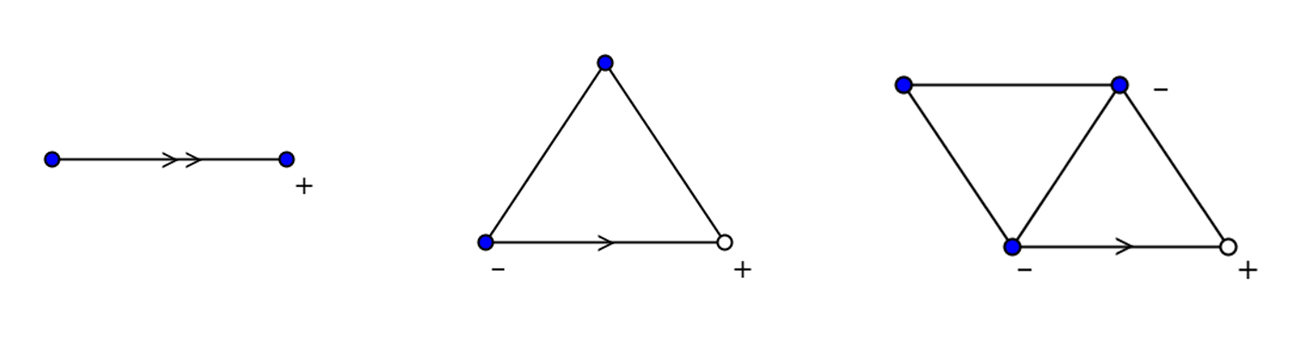
\includegraphics[width=0.6\textwidth]{pass.jpg}
\caption{Example of discharging rules (graphs made based on \cite{thomas1998update})}
\label{fig:pass}
\end{figure}

\begin{remark}
It seems that the way discharging method is used in the proof of the 4CT can be generalized and used to prove other statements that, like the 4CT, are not explicitly involved with reducible configurations.

Suppose we aim to prove a statement, "all graphs with property $P$ must have property $S$."

For purpose of contradiction, we suppose that there is a minimal counterexample with property $P$ that does not have property $S$. We can prove the result in two steps. First, argue that a minimal counterexample cannot have configurations $C_{1}$, or $ C_{2}$, or $C_{3}$..., because we can obtain a smaller counterexample otherwise. Second, show that configurations $C_{1}$, $ C_{2}$, $C_{3}$... are reducible for property $P$ using the discharging method. Combining the results of the two steps, we will obtain an contradiction. Therefore, there is no minimal counterexample of the result we aim to prove.
\end{remark}


\section{Conclusion}
As we have seen, the discharging rules allow charge to flow between adjacent vertices, or between incident faces and vertices. This process and its local results seem to shed light on the global property of a graph. 

Discharging is a very unique and useful proving technique, which in its core is a proof by contradiction. This essay, as an introduction to discharging, has only covered a shallow and narrow range of the application of discharging. Far more could be said on this very interesting topic.



%------------------------------------------------

%----------------------------------------------------------------------------------------
%	BIBLIOGRAPHY
%----------------------------------------------------------------------------------------

\bibliographystyle{acm}

\bibliography{sample}

%----------------------------------------------------------------------------------------

\end{document}